
\documentclass[journal]{IEEEtran}


\ifCLASSINFOpdf
  \usepackage[pdftex]{graphicx}
  \DeclareGraphicsExtensions{.pdf,.jpeg,.png}
\else

\fi
\usepackage[justification=centering]{caption}

\usepackage{amsmath}
\usepackage{amssymb}
\usepackage{float}
\usepackage{graphicx}
\usepackage{algorithm}
\usepackage{algorithmic}

\usepackage[strings]{underscore}
\usepackage{url}
\usepackage{enumerate}

\hyphenation{op-tical net-works semi-conduc-tor}


\begin{document}

\title{V-REP Integrated Paparazzi Simulation\\}


\author{Dominik Weikert}% <-this % stops a space


\maketitle


\begin{abstract}
This paper describes a framework for integrating the native paparazzi control-loop for UAVs into the 3D virtual-robot experimentation platform v-rep, created for the simulation of the quadricopters in the Otto-Von-Guericke University swarmlab. 
\end{abstract}

% Note that keywords are not normally used for peerreview papers.
%-%\begin{IEEEkeywords}
%-%IEEE, IEEEtran, journal, \LaTeX, paper, template.
%-%\end{IEEEkeywords}






% For peer review papers, you can put extra information on the cover
% page as needed:
% \ifCLASSOPTIONpeerreview
% \begin{center} \bfseries EDICS Category: 3-BBND \end{center}
% \fi
%
% For peerreview papers, this IEEEtran command inserts a page break and
% creates the second title. It will be ignored for other modes.
\IEEEpeerreviewmaketitle



\section{Introduction}

The OVGU swarmlab is a robotic lab in which experiments applying the theory of swarm intelligence are performed, mainly using custom-built quadricopters called FINken. To complement the live experiments, a 3D simulation software was needed. Simulation allows for faster creation of experimental data and reduces the risk of severely damaging the copters in the lab. The real FINken in the swarmlab use paparazzi, an open-source software for the control of multicopters and other UAVs. As paparazzi already provides a Simulator, the New Paparazzi Simulator (NPS), which allows custom back-ends to provide a flight dynamics model (FDM), it seemed the best do create such a back-end to integrate into the customizable virtual robot experimentation platform V-REP. This provides the advantage of implicit portability between the real FINken running paparazzi and the V-REP - paparazzi simulation.
To this end, a custom VREP-plugin was developed in C++ to enable the exchange of data between the two programs.
This paper describes the basic architecture of the framework created to establish this, and provides some evaluation data on the accuracy of the V-REP simulation loop.



\section{Framework Architecture}

The base of the combined Simulator is founded on a client-server architecture, with the paparazzi controller acting as a client to the VREP-plugin. In the FDM of the paparazzi simulator, a connection to a server representing the controlled simulated copter in V-REP is established. Using a multi-threaded model, multiple copters could be simulated at any point in time. Once the connection is established, simple data packets are exchanged containing the necessary data for each side:
Paparazzi provides data regarding the commands for the control of the FINken-motors, while V-REP provides data regarding the position and attitude of the FINken needed in the FDM to compute those controls.

\subsection{V-REP plugin}

The V-Rep plugin is responsible for providing the server architecture as well as handling the data on any individual FINken and synchronization between them.
To this end, each incoming client connection is paired (via ID) with a compatible FINken in the V-REP scene. This FIN-ken object can then run in a separate thread to obtain its commands, update its position and send its new position to the paparazzi client. Meanwhile the plugin ensures that all FINken have received (or sent) their data before the simulation can continue.
The basic loop in the plugin thus consists of the following steps:

\begin{enumerate}[\textbf{ }1:]
	\item Receive commands from the paparazzi client
	\item Apply commands to the copters
	\item Wait for all copters to update their position
	\item Send new positions to the paparazzi client
\end{enumerate}


\subsection{Paparazzi back-end}

As described above, the paparazzi client is responsible for receiving the copter data, passing it to the paparazzi simulator and sending the new commands to the V-REP plugin. 

When the position and attitude data is received, it is converted from the V-REP coordinates, which are in the NED system, to
the correct coordinate systems used in paparazzi, mainly ENU and ECEF. Paparazzi already provides several data structures and converters to accomplish this. Once those data structures are filled correctly, the paparazzi simulation can advance and calculate the next commands to send to the V-REP plugin. Afterwards, the client blocks the advancement of the NPS until new attitude data is received. To keep the simulations in time-sync, paparazzi also receives the time-step set in the V-REP simulation and the simulation time is manually advanced using that time-step.



\section{Test flights}

\begin{figure}	
	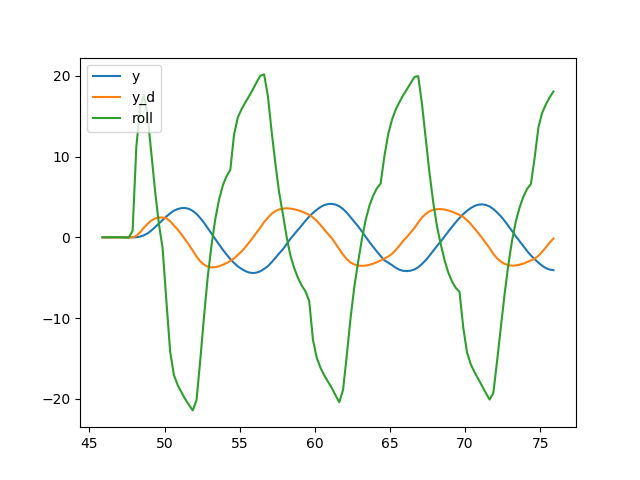
\includegraphics[width=0.5\textwidth]{logplots/straight-y.png}
	\caption{Test-flight 1: straight line on x axis}
	\label{flight1}
\end{figure}
This section shows some plots of recorded position data during simple test flight plans.
The the first test flight is on a horizontal line between points 10m apart. The results are shown in Fig \ref{flight1}.





\section{Acknowledgement}




%\bibliographystyle{IEEEtran}

%\bibliography{mybib}{}




\end{document}


